\documentclass[
    a4paper,
    12pt,
    parskip=half,
    bibliography=totoc,
]{scrartcl}
\usepackage[utf8]{inputenc}

\usepackage{imakeidx}
\indexsetup{othercode=\footnotesize,level=\section*,firstpagestyle=headings}
\makeindex[options=-s cnltx.ist,intoc]

\usepackage[
    typ=pub,
    link=LaTeX.dlrg.de,
    module={Personenicon,Paketbeschreibung}
]{dlrg}
\usepackage[
    language=ngerman,
    backend=biber,
    sortlocale=de_DE,%.UTF-8
    style=authoryear,
    bibencoding=UTF8,
    block=space,
    autocite=inline % \autocite[..][..]{..} erzeugt Literaturverweise mit runden Klammern
]{biblatex}
\usepackage{listings}
\usepackage{todonotes}
\usepackage{standalone}
\usepackage{subcaption}

\title{\LaTeX{}-Paket für die DLRG}
\author{Johannes Pieper}

\addbibresource[type=file]{dlrg.bib}
\lstset{%
    breaklines=true, % Zeilenumbrüche
    language=[latex]tex,
    basicstyle=\ttfamily\small,
    breakatwhitespace=false,
}

\makeatletter
\titelExtra{
    \vfill
    \begin{large}
        \begin{tblr}{colspec={lX[l]}, width=.5\textwidth}
            Version: & 1.1.0\\
            Datum: & \@date\\
            Betreuer: & \@author\\
        \end{tblr}
    \end{large}
}

\begin{document}

\maketitle

\tableofcontents

\clearpage

\section{Vorwort}
    Mit dem Handbuch Corporate Design (\cite{DLRG_CD2024}) hat die DLRG festgelegt, wie das Aussehen von verschiedenen Elementen zu gestalten ist, die mit der Öffentlichkeit in Berührung kommen. Dazu gehören auch Briefe, Broschüren und Präsentation, die sich auch mit \LaTeX{} erstellen lassen. Hier setzt dieses Paket an, dass neben den nötigen Umsetzungen auch Beispiele mitliefert.

    Besonders durch die komplett ehrenamtliche Erstellung dieses Paket erhebt es keinen Anspruch auf Vollständigkeit und Richtigkeit. Entsprechend ist jeder Verbesserungsvorschlag und jede Ergänzung herzlich willkommen. Dieses ist über \url{https://gitlab.com/dlrg-fs/dlrg_latex/-/issues} möglich. Die Quellen dieses Pakets sind als Git unter \url{https://gitlab.com/dlrg-fs/dlrg_latex} verfügbar.

    \subsection{Öffentliche Version und Markenrecht}\label{sec:markenrecht}
    Die Wort- und Bildmarke der DLRG sind markenrechtlich geschützt. Sie dürfen nur im Auftrag der DLRG Gliederungen verwendet werden. Dieses schließt auch den angeschnittenen Adler mit ein. Aus diesem Grund enthält das Paket nur in den bereits gesetzten Dokumenten diese geschützten Elemente. Für das fehlerfreie Setzen eigener Dokumente mit diesem Paket sind Platzhalter beigefügt. Das Aussehen davon ist im Anhang unter \nameref{sec:platzhalter} dargestellt.

    Im Internet-Service-Center (\url{dlrg.net}) haben Mitglieder der DLRG die Möglichkeit über die Dokumenten-App die Markenelemente herunterzuladen. Sie sind direkt über \url{https://k.dlrg.de/latex_elemente} zu erreichen. Dort ist auch eine Installationsanleitung unter \url{https://k.dlrg.de/latex_anleitung} dafür zu finden.

    \subsection{Beteiligte Personen}
    Besonderen Dank gilt folgenden Personen, die durch Anregungen, Hinweise und Ergänzungen zu diesem Paket beigetragen haben:
    \begin{itemize}
        \item Jonas Kipfstuhl
        \item Niklas Reimer
        \item Christoph Runge
    \end{itemize}


\section{Aufbau des Pakets}
    Das Paket gliedert sich in zwei verschiedene Elemente. Zum einen kann ein einzelner Dokumenttyp gewählt werden. Zu jedem Dokumententyp können verschiedene Module zusätzlich geladen werden. Einige Typen laden bereits einzelne Module automatisch.

\section{Dokumententypen}
    Über den Dokumententyp wird ausgewählt, welche Art von Dokument im Bezug zur DLRG genutzt werden soll. Den Typ gibt man über die Option \option{typ} beim Einbinden des Pakets an. Aktuell stehen \pkg{beamer} für Präsentationen, \pkg{pub} für Publikationen und \pkg{letter} für Briefe zur Verfügung.
    \begin{options}
        \keyval{typ}{Typname}\Default Der Typ wird mit seinem Namen angegeben
    \end{options}

\begin{sourcecode}
    \usepackage[
        typ=beamer
    ]{dlrg}
\end{sourcecode}

    \subsection{Präsentation}
        \documentclass[
    a4paper,
    12pt,
    parskip=half,
]{scrartcl}
\usepackage[utf8]{inputenc}

\usepackage[
    typ=pub,
    link=dlrg.net,
    module={Paketbeschreibung}
]{dlrg}
\usepackage{listings}
\usepackage{todonotes}
\usepackage{standalone}

\title{\LaTeX{}-Paket für die DLRG}
\subtitle{Abschnitt Präsentation}
\author{Johannes Pieper}

\begin{document}
    Ein Präsentation ist der Typ \verbcode|beamer| anzugeben. Die Präsentation besteht aus einer Startfolie, wie in \autoref{fig:vortrag_startfolie} zu sehen, und beliebig vielen Unterseiten.  Die Angaben im Fuß jeder Folie sind individuell einstellbar.

    \begin{figure}[ht]
        \centering
        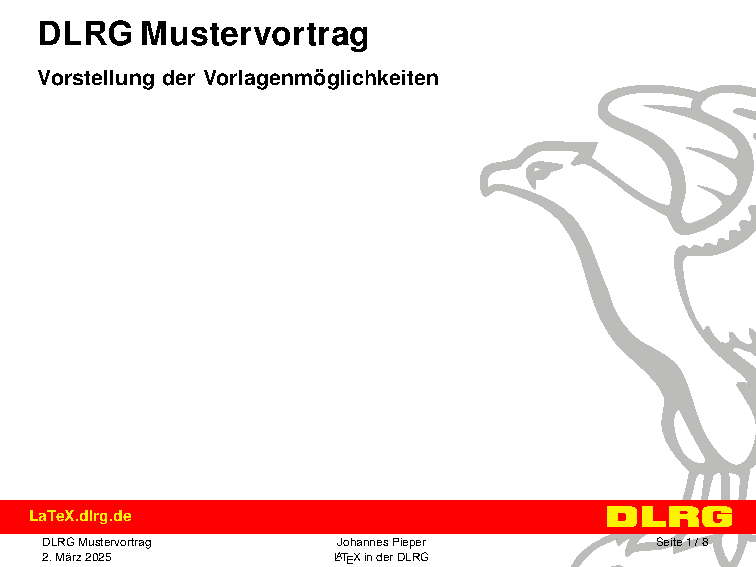
\includegraphics[width=0.7\linewidth]{Beispiele/dlrg_muster_vortrag}
        \caption{Startfolie des Mustervortrags}
        \label{fig:vortrag_startfolie}
    \end{figure}

    \subsubsection{Titelfolie}
        Die Titelfolie im passenden Design wird einfach über den Befehl \verbcode{\titlepage} gesetzt. Titel und Untertitel der Präsentation lassen sich über die Standardbefehle vom Paket \pkg{beamer} einstellen.

        \begin{options}
            \keyval{titelbild}{Dateiname}\Default Das Hintergrundbild lässt sich darüber angeben. Wird diese Option nicht genutzt, erscheint der angeschnittene Adler auf der Startfolie.
            \keychoice{titelschriftfarbe}{black,white}\Default{black}
        \end{options}

        \begin{commands}
            \command{title}[\marg{Titel}] Standardbefehl von \pkg{beamer} für den Titel der Präsentation.
            \command{subtitle}[\marg{Untertitel}] Standardbefehl von \pkg{beamer} für den Untertitel der Präsentation.
        \end{commands}

        \begin{sourcecode}[gobble=12]
            \begin{frame}
                \titlepage
            \end{frame}
        \end{sourcecode}

    \subsubsection[Folienfuß]{Angaben im Folienfuß}
        Im Fuß aller Folien werden verschiedene Angaben aufgeführt. Dieses lassen sich teilweise über Befehle von \pkg{beamer} angeben und teilweise sind eigene hinzugekommen. Wird der Link nicht explizit angegeben, so erscheint \code{dlrg.de}.

        \begin{commands}
            \command{author}[\marg{Name}] Der Name des Autors oder der Autoren.
            \command{institute}[\marg{Gliederung}] Hier lässt sich z.\,B. die Gliederung angeben.
            \command{date}[\marg{Datum}] Das Datum für die Präsentation.
            \command{footerLink}[\marg{Link}] Der Link z.\,B. zur Gliederung. Es ist dabei zu beachten, dass \textbf{kein} www. vorangestellt werden darf.
        \end{commands}

    \subsubsection{Format der Folien}
        Standardmäßig werden die Folien der Präsentation im 4:3-Format gesetzt. Das 16:9 Format lässt sich nur direkt als Option für den Dokumententyp \pkg{beamer} einstellen. Die Entsprechende Option lautet \keyis{aspectratio}{169}.

        \begin{sourcecode}[gobble=12]
            \documentclass[aspectratio=169]{beamer}
        \end{sourcecode}

\end{document}


    \subsection{Brief}
        \documentclass[
    a4paper,
    12pt,
    parskip=half,
]{scrartcl}
\usepackage[utf8]{inputenc}

\usepackage[
    typ=pub,
    link=dlrg.net,
    module={Paketbeschreibung}
]{dlrg}
\usepackage{listings}
\usepackage{todonotes}
\usepackage{standalone}

\title{\LaTeX{}-Paket für die DLRG}
\subtitle{Abschnitt Brief}
\author{Johannes Pieper}

\begin{document}
    Zur Darstellung eines Briefs im Layout der DLRG dient der Typ \verbcode|letter| als Vorlage. Die Angaben für den Briefkopf und Fuß werden über verschiedene Befehle getätigt. Als Dokumentenklasse muss \verbcode|scrlttr2| gewählt werden.

    \subsubsection{Briefkopf}
        Der Briefkopf besteht aus der Rücksendeadresse über dem Empfänger und der kompletten Adresszeile. Bei beiden werden der Gliederungsname, die Adresse und der Ort mit angegeben. Beim Gliederungsnamen ist es möglich, für die Rücksendeadresse eine Version anzugeben, bei der die Gliederungsbezeichnung abgekürzt wird.

        \begin{commands}
            \command{gliederungName}[\oarg{Kurzversion}\marg{Glederungsname}] Der Gliederungsname mit Bezeichnung wie "`Ortsgruppe Muster"'. Optional läst sich der Gliederungsname oberhalb der Empfängeradresse auch abkürzen zu "`OG Muster"'.
            \command{funktionsbezeichnung}[\marg{Funktion}] Angabe der Funktion in der Gliederung, wie "`Leiter Einsatz"'.
            \command{ansprechpartner}[\marg{ansprechpartner}] Name des Ansprechpartners in der angegebenen Funktion.
            \command{adresseZusatz}[\marg{Adresszusatz}] Angabe eines Zusatzes über der Adresse. Dieses könnte die Angabe Geschäftsstelle oder Hauptwache sein.
            \command{adresse}[\marg{Adresse}] Adresse aus Straße und Hausnummer.
            \command{ort}[\marg{Ort}] Angabe der Postleitzahl mit dem Ort.
            \command{telefon}[\marg{Telefonnummer}] Angabe der Telefonnummer. Am besten im Format "`+49 (0) 123 4567"'.
            \command{telefax}[\marg{Telefax}] Angabe einer Telefaxnummer. Format wie beim Telefon.
            \command{email}[\marg{email}] Die E-Mail-Adresse sollte komplett klein angeben werden.
            \command{webseite}[\marg{Internetadresse}] Die Angabe der Internetadresse sollte \textbf{ohne} führendes www. angegeben werden.
        \end{commands}

    \subsubsection{Betreff und und weiteres}
        Der eigentliche Inhalt des Briefs wird direkt im Dokument als Fließtext angegeben. Für den Betreff steht ein passender Befehl zur Verfügung. Unter der Grußformel wird automatisch die Signatur aus Ansprechpartner und seiner Funktionsbezeichnung ergänzt. Soll diese anders lauten, kann auch dieses abgeändert werden.

        \begin{commands}
            \command{betreff}[\marg{Betreff}] Der Betreffs des Briefes.
            \command{signatur}[\marg{Signatur}] Alternative Signatur, wenn diese nicht mit dem Ansprechpartner und seiner Funktionsbezeichnung übereinstimmt.
        \end{commands}

    \subsubsection{Fußzeile}
        Die ausführliche Fußzeile wird nur auf der ersten Seite des Briefes angegeben. Sollte der Brief aus mehreren Seiten bestehen, so haben alle folgenden Seiten nur die Seitenzahl in der Fußzeile stehen. Für die Angaben in der Fußzeile stehen folgende Befehle zur Verfügung:

        \begin{commands}
            \command{bankverbindung}[\marg{Bank}] Angaben zur Bankverbindung.
            \command{rechtsform}[\marg{Rechtsform}] Angabe zur Rechtsform der Gliederung.
            \command{gericht}[\marg{Gerichtsort und Nummer}] Angabe des Gerichts, bei dem die Gliederung registriert ist.
            \command{bgbVorstand}[\marg{Vorstand}] Angabe des Vorstandes nach §\,26 BGB. Die einzelnen Personen sollten durch Zeilenumbruch getrennt werden.
            \command{bankverbindung}[\marg{Bankverbindung}] Die Angabe der Bankverbindung. IBAN und Bankname sollte durch Zeilenumbruch getrennt werden.
        \end{commands}

\end{document}

    \subsection{Publikation}
        \documentclass[
    a4paper,
    12pt,
    parskip=half
]{scrartcl}
\usepackage[utf8]{inputenc}
\usepackage[
    typ=pub,
    link=dlrg.net,
    contentLayout=bauchbinde,
    module={Paketbeschreibung}
]{dlrg}
\usepackage[
    language=ngerman,
    backend=biber,
    sortlocale=de_DE,%.UTF-8
    style=authoryear,
    bibencoding=UTF8,
    block=space,
    autocite=inline % \autocite[..][..]{..} erzeugt Literaturverweise mit runden Klammern
]{biblatex}
\usepackage{listings}
\usepackage{todonotes}
\usepackage{standalone}

\title{\LaTeX{}-Paket für die DLRG}
\subtitle{Abschnitt Publikation}
\author{Johannes Pieper}

\begin{document}
Der Dokumententyp \verbcode|pub| ist die Kurzform für Publikationen und zur Zeit die Standardeinstellung für Dokumntentypen des DLRG-Pakets. Dieser diese mehrseitigen Publikationen können z.\,B. Handbücher oder Regelwerke sein. Als Dokumentenklasse empfiehlt sich der Einsatz von \verbcode|scrartcl|.

\subsubsection{Layout}
Um das Layout dieser Publikation zu beeinflussen gibt es mehrere Optionen, die beim Paket mit angegeben werden können.
\begin{options}
    \keychoice{contentLayout}{bauchbinde,footline}\Default{footline}
        Über diese Option lässt sich das Gesamtlayout einstellen.
        Bei der ersten Möglichkeit bekommt jede Seite eine Bauchbinde. Die zweite Möglichkeit hat die einfache Wortmarke in der Fußzeile und ist gemäß CD-Handbuch \autocite[S.~13]{DLRG_CD2019} angelegt. Sie ist standardmäßig aktiviert.
    \keyval-{titelbild}{Dateiname}
        Wenn ein seitenfüllendes Titelbild eingebunden werden soll, so ist über diese Option der Dateiname anzugeben. Wird nichts angegeben erscheint der halbe Adler als Wasserzeichen auf der Titelseite
    \keyval{titelbildcaption}{Text}
        Ist ein Titelbild angegeben, so lässt sich hierrüber ein Bildtitel und damit auch ggf. verbunden der Verweis auf den Fotograph. Dieses wird dann in einem möglichen Abbildungsverzeichnis mit aufgeführt.
\end{options}

Zusätzlich kann die Titelseite nach eigenen Wünschen ergänzt werden. Auch kann das Format der Seite im Dokument gedreht werden.

\begin{commands}
    \command{titelExtra}[\marg{Titelelemente}] Ermöglicht auf der Titelseite weitere Elemente zu platzieren. Diese müssen als Parameter übergeben werden.
    \command{querformatSeite}
        Dreht das Standardmäßig als Hochformat eingestellt Format der Seite auf Querformat.
    \command{hochformatSeite}
        Dreht das Seitenformat wieder auf Hochformat zurück.
\end{commands}

\subsubsection{Boxen}
\begin{environments}
    \environment{redPartBox}
    Erzeugt eine rot umrandete Box, die Zwischenüberschriften enthalten kann.
    \begin{commands}
        \command{partTitle}[\marg{Überschrift}]
        Setzt die Zwischenüberschrift der \verbcode|redPartBox|.
    \end{commands}
    \begin{example}[gobble=8]
        \begin{redPartBox}
            \partTitle{Teil1}
            Etwas Text
            \partTitle{Teil2}
            Etwas mehr Text
        \end{redPartBox}
    \end{example}
\end{environments}
\end{document}


    \subsection{Mitteilung}
        \documentclass[
    a4paper,
    12pt,
    parskip=half,
]{scrartcl}
\usepackage[utf8]{inputenc}

\usepackage[
    typ=pub,
    link=dlrg.net,
    module={Paketbeschreibung}
]{dlrg}
\usepackage{listings}
\usepackage{todonotes}
\usepackage{standalone}

\title{\LaTeX{}-Paket für die DLRG}
\subtitle{Abschnitt Mitteilung}
\author{Johannes Pieper}

\begin{document}
    Mit dem Dokumenttyp \verbcode|message| gibt es die Möglichkeit einfach gestaltete Mitteilungen zu gestalten, wie z.\,B. Pressemitteilungen, wie sie in \autoref{fig:mitteilung} dargestellt ist.
    \begin{figure}[ht]
        \centering
        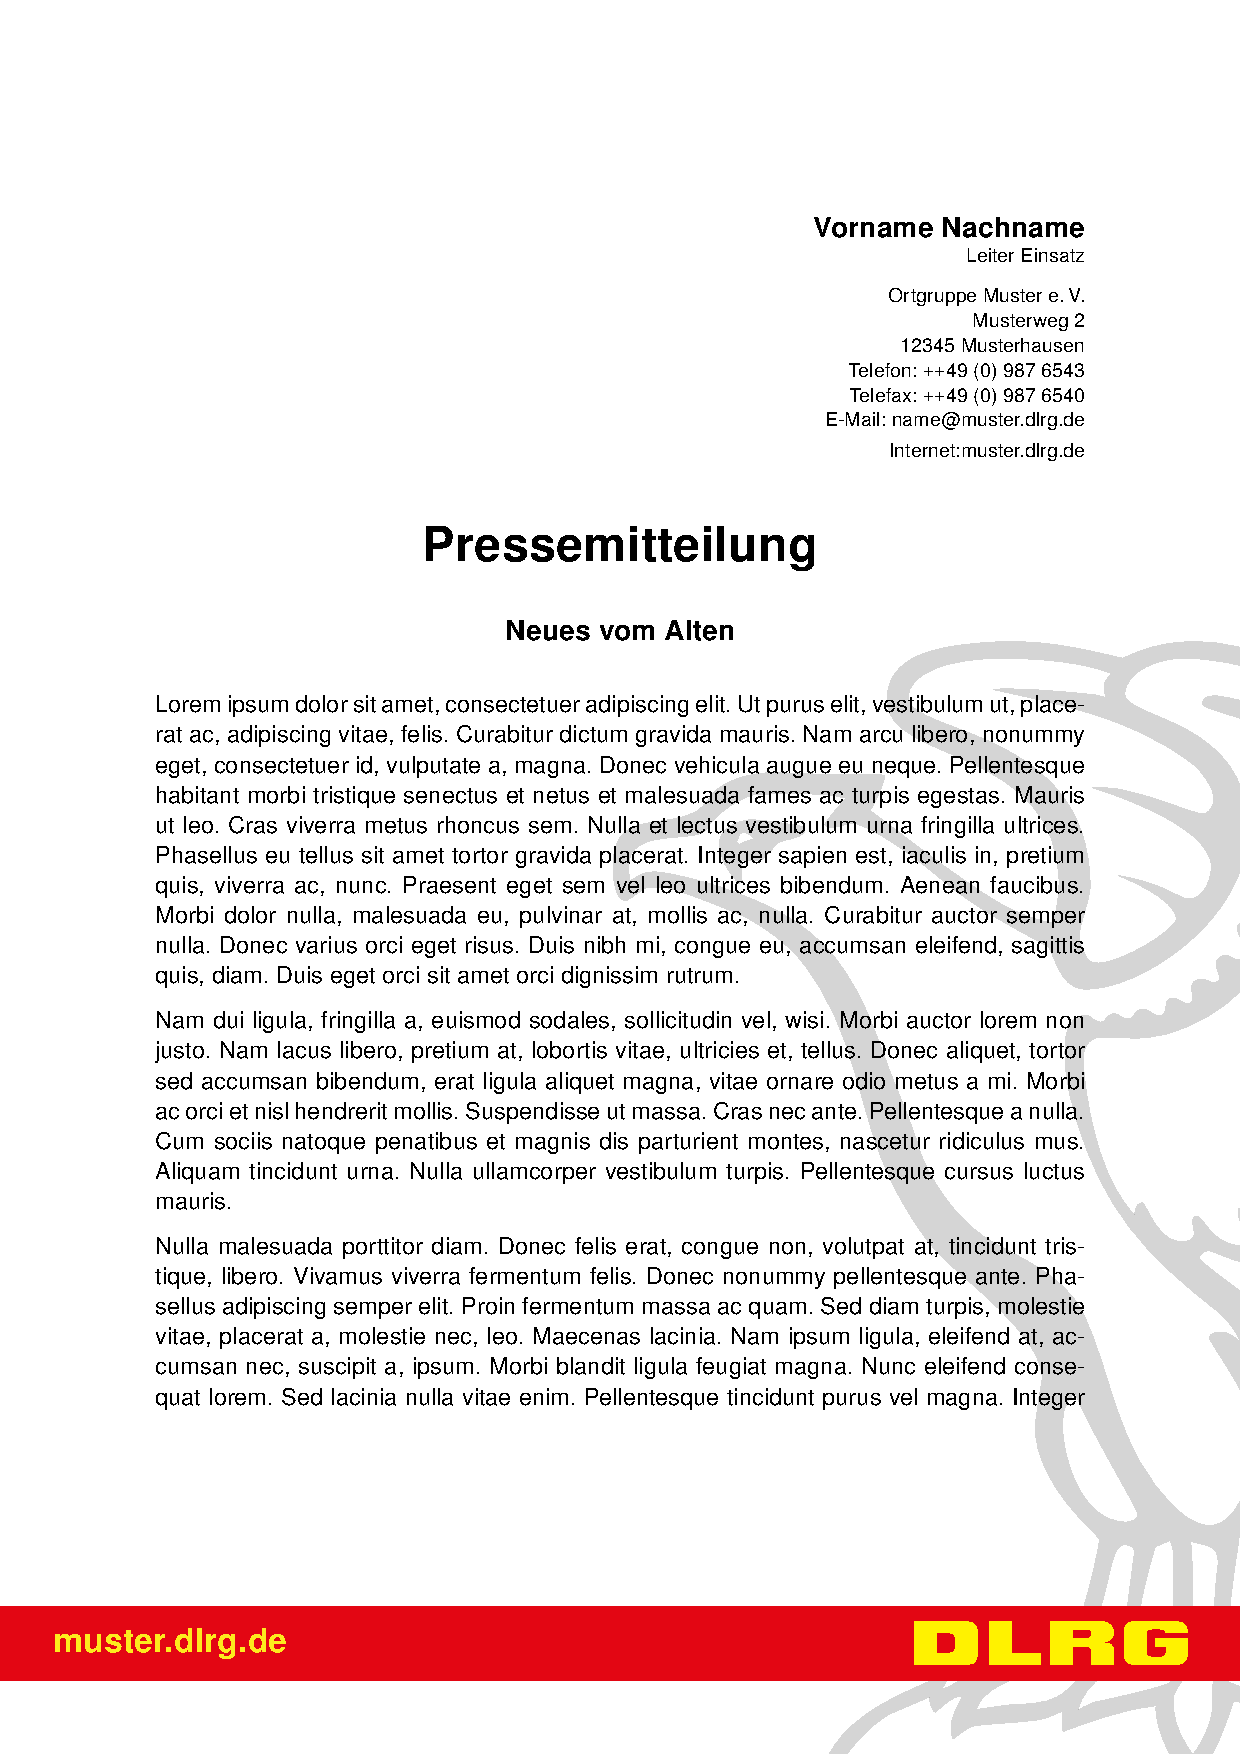
\includegraphics[scale=0.4]{Beispiele/dlrg_muster_mitteilung}
        \caption{Beispiel einer Mitteilung}
        \label{fig:mitteilung}
    \end{figure}

    \begin{commands}
        \command{titel}[\marg{Titel}] Der Titel der Mitteilung.
        \command{subtitle}[\marg{Untertitel}] Der Untertitel einer Mitteilung.
        \command{author}[\marg{Autor}] Der Autor der Mitteilung.
        \command{gliederungName}[\marg{Glederungsname}] Der Gliederungsname mit Bezeichnung wie "`Ortsgruppe Muster"'.
        \command{funktionsbezeichnung}[\marg{Funktion}] Angabe der Funktion des Autors in der Gliederung, wie "`Leiter Einsatz"'.
        \command{adresse}[\marg{Adresse}] Adresse aus Straße und Hausnummer.
        \command{ort}[\marg{Ort}] Angabe der Postleitzahl mit dem Ort.
        \command{telefon}[\marg{Telefonnummer}] Angabe der Telefonnummer. Am besten im Format "`+49 (0) 123 4567"'.
        \command{telefax}[\marg{Telefax}] Angabe einer Telefaxnummer. Format wie beim Telefon.
        \command{email}[\marg{email}] Die E-Mail-Adresse sollte komplett klein angeben werden.
        \command{webseite}[\marg{Internetadresse}] Die Angabe der Internetadresse sollte \textbf{ohne} führendes www. angegeben werden. Diese Adresse wird auch in der Bauchbinde genutzt.
    \end{commands}

    \subsubsection{Serienfunktion}
    Für den Fall, dass man die Mitteilung durch eine Serienfunktion, wie sie z.\,B. mit dem Paket \pkg{datatool} bereit gestellt wird, muss man den Kopf mit hinterlegten Adler durch \verb|\startMitteilungsteil| selbst einbinden. Will man
    den ersten Kopf unterdrücken, so kann man dieses durch die Option \verb|serienfunktion| machen.

    \begin{options}
        \opt{serienfunktion}
            Mit der aktivierten Serienfunktion wird die automatische Einbindung des Kopfes unterbunden.
    \end{options}

    \begin{commands}
        \command{startMitteilungsteil} Setzt einen neuen Kopf mit hinterlegtem Adler. Auch wird ein Seitenumbruch zuvor durchgeführt.
    \end{commands}

\end{document}


\section{Module}
    Die Module des Paketes werden teilweise automatisch durch die verschiedenen Dokumententypen geladen. Alle Module lassen sich auch immer optional hinzuladen oder auch ohne einen Dokumententyp laden. Das Laden von Modulen funktioniert über die Optionen an das Paket.

    \begin{options}
        \keyval{module}{Modul1,Modul2,\dots}\Default Weitere Module können geladen werden, indem sie der Paketoption \option{module} als kommaseparierte Liste übergeben werden.
    \end{options}


    \subsection{Bauchbinde}
        \documentclass[
    a4paper,
    12pt,
    parskip=half,
]{scrartcl}
\usepackage[utf8]{inputenc}

\usepackage[
    typ=pub,
    link=LaTeX.dlrg.de,
    module={Paketbeschreibung,Tabellen}
]{dlrg}
\usepackage{listings}
\usepackage{standalone}
\usepackage[
    language=ngerman,
    backend=biber,
    sortlocale=de_DE,%.UTF-8
    style=authoryear,
    bibencoding=UTF8,
    block=space,
    autocite=inline % \autocite[..][..]{..} erzeugt Literaturverweise mit runden Klammern
]{biblatex}

\title{\LaTeX{}-Paket für die DLRG}
\subtitle{Abschnitt Bauchbinde}
\author{Johannes Pieper}

\begin{document}
    Dieses Modul wird von fast jedem bereits automatisch eingebunden. Mit ihm lässt sich die Bauchbinde, die typisch ist für Dokumente der DLRG, setzen. In vielen Fällen hat diese im linken Bereich einen Link, dieser lässt sich als Option an das Paket anpassen.

    \begin{options}
        \keyval{link}{Link}\Default{dlrg.de}
            Gibt den Link an, der in der Bauchbinde an der linken Seite dargestellt werden soll.
    \end{options}

    Die eigentliche Einbindung erfolgt über einen Befehl:

    \begin{commands}
        \command{bauchbinde}[\sarg]
            Setzt die Bauchbinde auf der Seite. Bei der Nutzung der Stern-Variante wird der Link im linken Bereich der Bauchbinde nicht angezeigt.
    \end{commands}
\end{document}


    \subsection{Schriftart}
        \documentclass[
    a4paper,
    12pt,
    parskip=half,
]{scrartcl}
\usepackage[utf8]{inputenc}

\usepackage[
    typ=pub,
    link=dlrg.net,
    module={Paketbeschreibung}
]{dlrg}
\usepackage{listings}
\usepackage{todonotes}
\usepackage{standalone}

\title{\LaTeX{}-Paket für die DLRG}
\subtitle{Abschnitt Schriftart}
\author{Johannes Pieper}

\begin{document}
Das CD der DLRG sieht vor, dass alle Schriftstücke möglichst mit der DLRG-Hausschrift verfasst werden. Dieses ist aber nur mit LuaTeX möglich. Dazu muss die Schrift auf dem System installiert sein. Das Modul bindet sie dann automatisch ein. Mit \LaTeX{} ist dieses nicht möglich.

Die Schrift kann im Internet Service Center der DLRG im \href{https://dlrg.net/apps/dokumente?page=assetService&noheader=1&aid=1709&v=o&file=DLRG%20Schriftart.zip}{Bereich der Dokumente } heruntergeladen werden. Dazu muss man mit einem bestätigten DLRG-Account angemeldet sein.

\subsubsection{DLRG-Schriftart mit \LaTeX}
Die Konvertierung in ein passendes \LaTeX{} Format ist nicht einfach. Außerdem ist Schriftart nicht öffentlich verfügbar, so dass aus lizensrechtlichen Gründen auch die Weitergabe der Konvertierung wahrscheinlich nicht zulässig ist. Als Alternative wird die Schriftart Arial aufgeführt. Alle Schriftstücken, die mit diesem Paket und \LaTeX{} erstellt werden, verwendet diese. Realisiert wird dieses durch das Paket uarial, dass ggf. noch installiert werden muss.

Die Installation von uarial kann bei TeX Live mit folgenden Schritten erfolgen:
\begin{enumerate}
    \item Zuerst muss eine Datei heruntergeladen werden: \\
        \url{http://tug.org/fonts/getnonfreefonts/install-getnonfreefonts}
    \item Unabhängig vom Betriebssystem muss diese mit \verbcode|texlua| ausgeführt werden:
    \begin{sourcecode}[gobble=8]
        texlua install-getnonfreefonts
    \end{sourcecode}
    \item Systemweit kann dann die Schriftart mit folgendem Aufruf installiert werden:
    \begin{sourcecode}[gobble=8]
        getnonfreefonts --sys arial-urw
    \end{sourcecode}
\end{enumerate}

Bei einem Wechsel der TexLive-Version muss man nur die Schrift wieder neu einbinden. Dieses geschieht durch Aufruf von:
\begin{sourcecode}[gobble=4]
    updmap-sys --enable Map=ua1
\end{sourcecode}

\end{document}


    \subsection{Tabellen}
        \documentclass[
    a4paper,
    12pt,
    parskip=half,
]{scrartcl}
\usepackage[utf8]{inputenc}

\usepackage[
    typ=pub,
    link=LaTeX.dlrg.de,
    module={Paketbeschreibung,Tabellen}
]{dlrg}
\usepackage{listings}
\usepackage{standalone}
\usepackage[
    language=ngerman,
    backend=biber,
    sortlocale=de_DE,%.UTF-8
    style=authoryear,
    bibencoding=UTF8,
    block=space,
    autocite=inline % \autocite[..][..]{..} erzeugt Literaturverweise mit runden Klammern
]{biblatex}

\title{\LaTeX{}-Paket für die DLRG}
\subtitle{Abschnitt Tabellen}
\author{Johannes Pieper}

\begin{document}
    Mit dem Paket \pkg{tabularray} gibt es in \LaTeX 3 eine umfassende Möglichkeit zur Gestaltung von Tabellen. Dieses wird automatisch mit dem Modul \module{Tabellen} eingebunden. Dadurch entfällt die Einbindung von \pkg{tabu}, was nicht mehr weiterentwickelt wird. Dieses war bis zur Version 0.2 über den Dokumentty \pkg{pub} für Publikationen eingebunden.

    Das Handbuch Corporate Design (\cite{DLRG_CD2024}) geht nicht näher darauf ein, wie Tabellen in Publikationen zu setzen sind. In verschiedenen Publikationen, die in der sogenannten Dokumenten-App im Internet-Service-Center zu finden sind, hat sich das Layout durchgesetzt, dass Tabellen mit schwarzen Rahmen umfasst sind und die Überschriften der Zeilen mit grauem Hintergrund belegt sind. Es folgt dafür ein passendes Beispiel.

    \begin{example}[gobble=8]
        \begin{tblr}{
            colspec={XXX[2]},
            vlines,hlines,
            row{1}={font=\bfseries,bg=gray!50}
        }
            Spalte 1 & Spalte 2 & Spalte 3 \\
            Inhalte & mehr Inhalte & Noch mehr Inhalte, die mehr sind \\
            Inhalt & wenig Inhalt & kurzer Inhalt \\
        \end{tblr}
    \end{example}

    Zur Vereinfachung für solche Tabellen ist die Umgebung \verb|dlrgTblr| geschaffen worden. Durch Optionen an diese Umgebung lassen sich auch Tabellen mit roten Linien und Überschriften erzeugen, wobei letztere dann zur Farbwahl der Linien passen. Zusätzlich zu den speziellen Optionen können auch optional äußere Einstellungen und die obligatorisch inneren Einstellungen, wie die Spaltenanzahl und Spaltenausrichtung mitgegeben werden, wie es aus dem \pkg{tabularray}-Paket bekannt ist.

    \begin{environments}
        \environment{dlrgTblr}[\oarg{Äußere Einsellungen}\marg{Innere Einsellungen} \oarg{Optionen}]
            Liefert eine auf \verbcode|tblr| basierende Tabelle im passenden DLRG-Layout. Entsprechend können alle Möglichkeiten davon genutzt werden. Diese Tabelle können zusätzlich über folgende Optionen angepasst werden:
            \begin{options}
                \keychoice*{layout}{grauSchwarz,rot}\Default{grauSchwarz}
                    Die DLRG Tabelle wird in zwei verschiedenen Layouttypen angeboten, wobei die Farbgebung sich auf die Kopfzeilen und Linienfarbe bezieht.
                \opt*{ueberschrift} Zeichnet die erste Zeile der Tabelle als Überschrift mit passender Hinterlegung und in fetter Schriftart.
                \opt*{noVlines} Verhindert das Zeichnen der vordefinierten vertikalen Linen recht und links an jeder Spalte in der Tabelle. Sie können aber immer noch auf normalem Wege gesetzt werden.
                \opt*{noHlines} Verhindert das Zeichnen der vordefinierten horizontalen Linien über und unter jeder Zeile. Sie können aber immer noch mit \verb|\hline| erzeugt werden.
                \opt*{long}
                    Macht aus der Tabelle eine Tabelle, die über mehrere Seiten gehen kann und dann passend getrennt wird.
            \end{options}
    \end{environments}

    Im folgenden ist die gleiche Tabelle wie oben mit diesen Optionen dargestellt.

    \begin{example}[gobble=8]
        \begin{dlrgTblr}{colspec={XXX[2]}}[ueberschrift]
            Spalte 1 & Spalte 2 & Spalte 3 \\
            Inhalte & mehr Inhalte & Noch mehr Inhalte, die mehr sind \\
            Inhalt & wenig Inhalt & kurzer Inhalt \\
        \end{dlrgTblr}
    \end{example}

    Auch mit der roten Variante soll diese Tabelle hier dargestellt werden.
    \begin{example}[gobble=8]
        \begin{dlrgTblr}{colspec={XXX[2]}}[ueberschrift,layout=rot]
            Spalte 1 & Spalte 2 & Spalte 3 \\
            Inhalte & mehr Inhalte & Noch mehr Inhalte, die mehr sind \\
            Inhalt & wenig Inhalt & kurzer Inhalt \\
        \end{dlrgTblr}
    \end{example}

    Neben der Tabelle wird auch noch ein Befehl zur Verfügung gestellt.
    \begin{commands}
        \command{tabellenZwischenueberschrift}[\marg{Spaltenanzahl}]
            Setzt eine Zwischenüberschrift über die angegebene Spaltenzahl als Zeile in eine DLRG-Tabelle. Der Inhalt der Zelle ist dann fett formatiert und linksbündig ausgerichtet.
    \end{commands}

    \subsubsection{Aufzählungen}
    Sollen in Tabellen Aufzählungen genutzt werden, so nehmen diese in der Regel sehr viel Raum ein und sprengen das Layout daher gibt es für Tabellen eine extra Möglichkeit für Aufzählungen, die daran angepasst sind.

    \begin{environments}
        \environment{tabellenItemize}
            Eine Aufzählungsumgebung, die innerhalb einer Tabelle genutzt werden kann und dabei möglichst kleine Abstände hat.
    \end{environments}
\end{document}


    \subsection{Hausarbeit Lehrschein}
        \documentclass[
    a4paper,
    12pt,
    parskip=half,
]{scrartcl}
\usepackage[utf8]{inputenc}

\usepackage[
    typ=pub,
    link=dlrg.net,
    module={Paketbeschreibung}
]{dlrg}
\usepackage{listings}
\usepackage{todonotes}
\usepackage{standalone}

\title{\LaTeX{}-Paket für die DLRG}
\subtitle{Abschnitt Hausarbeit}
\author{Johannes Pieper}

\begin{document}
Das Modul \module{Hausarbeit} wurde für die Erstellung einer solchen im Rahmen der Lehrscheinprüfung erstellt. Es bindet Elemente für die spezifischen Anforderungen ein, die für eine normale Publikation nicht gegeben sind.

\subsubsection{Moduloptionen}
Über die Moduloptionen lässt sich bei der Hausarbeit einstellen, ob die Hinweistexte, die in \autoref{sec:HausarbeitHinweise} näher beschrieben sind, angezeigt werden sollen oder nicht.

\begin{options}
    \keybool{hinweise}\Default{false}
        Gibt an, ob die Hinweise angezeigt werden.
        \label{option:hinweise}
\end{options}

\subsubsection{Titelseite}
Bei der Hausarbeit wird die Titelseite mit einem weiteren Störer versehen, der die weiteren nötigen Angaben enthält.

\begin{commands}
    \command{date}[\marg{Datum}]
    Der Standardbefehl für das Datum wird mit diesem Modul neu definiert.

    \command{author}[\marg{Autor}]
    Der Standardbefehl für den Autor des Dokuments wird mit diesem Modul neu definiert.

    \command{menor}[\marg{Mentor}]
    Mit diesem Befehl lässt sich der Mentor angeben, der auf der Startseite angegeben wird.

    \command{ort}[\marg{Ort}]
    Angabe für den Ort, der auf der Startseite mit angegeben wird.

    \command{thema}[\oarg{Kurzform des Themas}\marg{Thema}]
    Anstatt des Titels wird mit der Hausarbeit das Thema auf der Titelseite angegeben. Dieses lässt auch optional eine Kurzform zu, die alternativ zum Thema in der Kopfzeile jeder Seite aufgeführt wird.
\end{commands}

\subsubsection{Stichwortverzeichnis}
Alle Dokumente, die dieses Modul laden werden um Elemente des Stichwortverzeichnisses aus dem Paket \verbcode|glossaries| erweitert. Die Einbindung des Stichwortverzeichnis erfolgt dann an entsprechender Stelle durch folgenden Befehl:

\begin{sourcecode}
    \printglossary[type=\acronymtype,title=Abkürzungsverzeichnis,style=long]
\end{sourcecode}

Nach der ersten Übersetzung des Dokumentes müssen dann die folgende Befehle abgesetzt werden, damit das Stichwortverzeichnis auch mit Inhalt gefüllt wird. Dabei muss der Dokumentenname entsprechend angepasst werden.

\begin{sourcecode}
    makeindex -s Dokumentenname.ist -t Dokumentenname.alg -o Dokumentenname.acr Dokumentenname.acn
\end{sourcecode}

\subsubsection{Hinweise}\label{sec:HausarbeitHinweise}
Die Vorlage des Landesverbands Westfalen enthält einige Hinweise, zur Gliederung und Aufbau der Hausarbeit. Da es bei diesen sinnvoll sein kann, sie während der Erstellungsphase sichbar zu halten, können sie durch die Moduloption \verbcode|hinweise| \ref{option:hinweise} geschaltet werden.

\begin{commands}
    \command{HinweisZurVorlage}[\marg{Text}]
        Ein Hinweistext kann angegeben werden, der in einem extra Kasten genau an dieser Stelle dargestellt wird. Dieser wird nur dann dargestellt, wenn die Moduloption \verbcode|hinweise| angewählt ist.
\begin{sourcecode}
    \HinweisZurVorlage{
        Hier ist eine Hinweis, wie etwas umgesetzt werden soll.
    }
\end{sourcecode}
    \begin{tcolorbox}[
            colback=white,
            colframe=dlrgRot,
            fonttitle=\bfseries,
            title=Hinweis -- bei einer Nutzung als Vorlage bitte löschen oder deaktivieren
        ]
        Hier ist eine Hinweis, wie etwas umgesetzt werden soll.
    \end{tcolorbox}
\end{commands}
\end{document}


    \subsection{Personenicon}
        \documentclass[
    a4paper,
    12pt,
    parskip=half,
]{scrartcl}
\usepackage[utf8]{inputenc}

\usepackage[
    typ=pub,
    link=LaTeX.dlrg.de,
    module={Paketbeschreibung,Personenicon}
]{dlrg}
\usepackage{listings}
\usepackage{standalone}
\usepackage[
    language=ngerman,
    backend=biber,
    sortlocale=de_DE,%.UTF-8
    style=authoryear,
    bibencoding=UTF8,
    block=space,
    autocite=inline % \autocite[..][..]{..} erzeugt Literaturverweise mit runden Klammern
]{biblatex}

\title{\LaTeX{}-Paket für die DLRG}
\subtitle{Abschnitt Personenicon}
\author{Johannes Pieper}

\begin{document}
Das Modul \module{Personenicon} stellt verschiedene Icons bereit, mit der Personen in verschiedenen Kontext rund um die Arbeit der DLRG dargestellt werden können. Alle Icons lassen sich nur innerhalb von \verbcode|\tikz| oder einer \verbcode|tikzpicture|-Umgebung nutzen. Dabei lassen sich alle je nach Wunsch in der Größe verändern und in eine passende Richtung drehen. Außerdem lässt sich angeben, ob es sich um ein DLRG-Person mit roter Kleidung oder eine normale Person handelt. Teilweise ist auch die Angabe des Geschlechts möglich. Die Reihenfolge der Optionen hinter den Koordinaten ist dabei beliebig, wobei keine Leerzeichen dazwischen zulässig sind.

\begin{commands}
    \command{dlrgPersonStehend}[\sarg \darg{x,y} \eargChoices{r}{n,e,s,w,\meta{Winkel}} \earg{s}{Faktor}]
        Eine stehende Person \tikz{\dlrgPersonStehend (0,0)}.

    \command{dlrgPersonStehendArme}[\sarg \darg{x,y} \eargChoices{r}{n,e,s,w,\meta{Winkel}} \earg{s}{Faktor}]
        Eine stehende Person, bei der die Arme nach vorne und hinten gehen \tikz{\dlrgPersonStehendArme (0,0)}.

    \command{dlrgPersonStehendSitzend}[\sarg \darg{x,y} \eargChoices{r}{n,e,s,w,\meta{Winkel}} \earg{s}{Faktor}]
        Eine sitzende Person \tikz{\dlrgPersonSitzend (0,0)}.

    \command{dlrgPersonSchwimmenKraul}[\sarg \darg{x,y} \eargChoices{r}{n,e,s,w,\meta{Winkel}} \earg{s}{Faktor} \eargChoices{g}{w,m} \earg{e}{Equip\-ment}]
        Eine Person die Kraul schwimmt \tikz{\dlrgPersonSchwimmenKraul (0,0)}.

    \command{dlrgPersonSchwimmenBrust}[\sarg \darg{x,y} \eargChoices{r}{n,e,s,w,\meta{Winkel}} \earg{s}{Faktor} \eargChoices{g}{w,m} \earg{e}{Equip\-ment}]
        Eine Person die Brust schwimmt \tikz{\dlrgPersonSchwimmenBrust (0,0)}.
\end{commands}

Es folgen Beispiele für den Einsatz der verschiedenen Optionen, die abhängig vom genutzten Personenicon sind.

\begin{description}
    \item[Kleidung (\textasteriskcentered):] Ein Stern hinter dem Befehl und vor den Koordinaten sorgt dafür, dass die Person in roter Kleidung dargestellt wird.
\begin{example}
    \tikz{\dlrgPersonStehend* (0,0)}
\end{example}

    \item[Rotation (r):] Entweder wird die Blickrichtung mit der Himmelsrichtung (n,e,s,w) angeben oder dem Winkel zur Standardrichtung, die nach Osten gerichtet ist.
\begin{example}
    \tikz{\dlrgPersonStehend (0,0)r{n}}
\end{example}

    \item[Skallierung (s):] Es kann ein Skallierungsfaktors angegeben werden, mit dem dem die Person vergrößert bzw. verkleinert wird.
\begin{example}
    \tikz{\dlrgPersonStehend (0,0)s{0.6}}
\end{example}

    \item[Geschlecht (g):] Über die Möglichkeiten w und m lässt sich das Geschlecht der Person wählen. Standardmäßig ist daabei männlich gewählt.
\begin{example}
    \tikz{\dlrgPersonSchwimmenKraul (0,0)g{w}}
\end{example}

    \item[Equipment (e):] Die Person kann mit weiterem Equipment ausgestattet werden. Welches Equipment möglich ist, hängt von der gewählten Form der Person ab. Das p steht dabei für Pullboy.
\begin{example}
    \tikz{\dlrgPersonSchwimmenKraul (0,0)e{p}}
\end{example}

\end{description}
\end{document}


    \subsection{Adler}
        \documentclass[
    a4paper,
    12pt,
    parskip=half,
]{scrartcl}
\usepackage[utf8]{inputenc}

\usepackage[
    typ=pub,
    link=dlrg.net,
    module={Paketbeschreibung}
]{dlrg}
\usepackage{listings}
\usepackage{todonotes}
\usepackage{standalone}

\title{\LaTeX{}-Paket für die DLRG}
\subtitle{Abschnitt Adler}
\author{Johannes Pieper}

\begin{document}
    Das Modul \module{Adler} dient zur Darstellung des angeschnittenen Adlers. Dabei ist darauf zu achten, dass dieser immer nur von rechts blickend dargestellt werden darf. Außerdem darf nur die linken 50\,\% zu sehen, sowie die unteren 10\,\% müssen verdeckt sein.

    \begin{commands}
        \command{freigestellterAdlerWasserzeichen}[\oarg{TikZ-Optionen}\darg{Verschiebung}] Zeichnet den angeschnittenen Adler als Wasserzeichen passend auf ein DIN-A4-Blatt an die untere rechte Ecke. Bei der Verwendung von anderen Formaten kann die Verschiebung angepasst werden, so dass die Regeln bezüglich des Anschnitts gewährleistet sind. Es können optional weitere TikZ-Optionen übergeben werden.
        \command{freigestellterAdlerZeichnen}[\oarg{TikZ-Optionen}\darg{Verschiebung}\oarg{Farbe}] Zeichnet den kompletten Adler ohne Oval. Als ersten optionalen Parameter können TikZ-Optionen übergeben werden. Die Verschiebung muss angegeben werden, wobei der Adler mittig ausgerichtet ist. Der dritte Parameter ermöglicht eine andere Farbe, abweichend von schwarz. Das Anschneiden des Adlers muss selbstständig vorgenommen werden.
        \begin{example}[gobble=12]
            \begin{tikzpicture}[scale=0.2]
                \clip(0,-12) rectangle(-30,17);
                \freigestellterAdlerZeichnen[opacity=.2](0,0)[red]
            \end{tikzpicture}
        \end{example}
    \end{commands}
\end{document}

\appendix

\section{Marke und Platzhalter}\label{sec:platzhalter}
    Da im öffentlichen DLRG-Paket die Markenelemente (Wortmarke und Bildmarke) nicht vorhanden sein dürfen, sind diese durch Platzhalter ersetzt worden (Siehe \nameref{sec:markenrecht}). An dieser Stelle sind der Platzhalter und das Original der Marke gegenübergestellt.

    \begin{figure}[ht]
        \begin{subfigure}[c]{0.5\linewidth}
            \centering
            \scalebox{0.2}{
                \begin{tikzpicture}
                    %\draw(-16,16) rectangle(16,-16);
                    \draw(-16,16)[thick,red] rectangle(0,-12.8);
                    %\clip(-17,16) rectangle(0,-12.8);
                    \adlerPlatzhalterZeichnen{}{0,0}{dlrgSchwarz}
                \end{tikzpicture}
            }
            \subcaption{Platzhalter}
        \end{subfigure}
        \begin{subfigure}[c]{0.5\linewidth}
            \centering
            \scalebox{0.2}{
                \begin{tikzpicture}
                    %\draw(-16,16) rectangle(16,-16);
                    \draw(-16,16)[thick,red] rectangle(0,-12.8);
                    %\clip(-17,16) rectangle(0,-12.8);
                    \freigestellterAdlerZeichnen(0,0){dlrgSchwarz}
                \end{tikzpicture}
            }
            \subcaption{Original}
        \end{subfigure}
        \caption{Der freigestellter Adler mit der Markierung für den zulässigen Ausschnitt}
    \end{figure}

    \begin{figure}[ht]
        \begin{subfigure}[c]{0.5\linewidth}
            \centering
            \includegraphics{dlrg_wortmarke_rot_platzhalter.pdf}
            \subcaption{Platzhalter}
        \end{subfigure}
        \begin{subfigure}[c]{0.5\linewidth}
            \centering
            \includegraphics{dlrg_wortmarke_rot}
            \subcaption{Original}
        \end{subfigure}
        \caption{Die Wortmarke}
    \end{figure}

    \begin{figure}[ht]
        \begin{subfigure}[c]{0.5\linewidth}
            \centering
            \includegraphics[width=35mm]{dlrg_adler_platzhalter.jpg}
            \subcaption{Platzhalter}
        \end{subfigure}
        \begin{subfigure}[c]{0.5\linewidth}
            \centering
            \includegraphics[width=35mm]{dlrg_adler.jpg}
            \subcaption{Original}
        \end{subfigure}
        \caption{Die Bildmarke für z.\,B. die Briefvorlage}
    \end{figure}

\printbibliography[title=Literaturverzeichnis]

\printindex

% \listoftodos
\end{document}
